\documentclass[table]{beamer}
%[]中可以使用draft、handout、screen、transparency、trancompress、compress等参数

%指定beamer的模式与主题
\mode<presentation>
{
  \usetheme{Madrid}
%\usetheme{Boadilla}
%\usecolortheme{default}
%\usecolortheme{orchid}
%\usecolortheme{whale}
%\usefonttheme{professionalfonts}
}

%\usetheme{Madrid}
%这里还可以选择别的主题:Bergen, Boadilla, Madrid, AnnArbor, CambridgeUS, Pittsburgh, Rochester, Warsaw, ...
%有导航栏的Antibes, JuanLesPins, Montpellier, ...
%有内容的Berkeley, PaloAlto, Goettingen, Marburg, Hannover, ...
%有最小导航栏的Berlin, Ilmenau, Dresden, Darmstadt, Frankfurt, Singapore, Szeged, ...
%有章和节表单的Copenhagen, Luebeck, Malmoe, Warsaw, ...

%\usecolortheme{default}
%设置内部颜色主题(这些主题一般改变block里的颜色);这个主题一般选择动物来命名
%这里还可以选择别的颜色主题,如默认的和有特别目的的颜色主题default,structure,sidebartab,全颜色主题albatross,beetle,crane,dove,fly,seagull,wolverine,beaver

%\usecolortheme{orchid}
%设置外部颜色主题(这些主题一般改变title里的颜色);这个主题一般选择植物来命名
%这里还可以选择别的颜色主题,如默认的和有特别目的的颜色主题lily,orchid,rose

%\usecolortheme{whale}
%设置字体主题;这个主题一般选择海洋动物来命名
%这里还可以选择别的颜色主题,如默认的和有特别目的的颜色主题whale,seahorse,dolphin

%\usefonttheme{professionalfonts}
%类似的还可以定义structurebold,structuresmallcapsserif,professionalfonts

% 控制 beamer 的风格,可以根据自己的爱好修改
%\usepackage{beamerthemesplit} %使用 split 风格
%\usepackage{beamerthemeshadow} %使用 shadow 风格
%\usepackage[width=2cm,dark,tab]{beamerthemesidebar}

%插入音标
%\usepackage{tipa}
%\AtBeginDocument{
  %\renewcommand\textipa{\fontencoding{T3}\selectfont}
%}
%\AtBeginDocument{
  %\renewcommand\textipa[2][r]{{\fontfamily{cm#1}\tipaencoding #2}}
%}
%\renewenvironment{IPA}[1][r]
 %{\fontfamily{cm#1}\tipaencoding}
 %{}

% 设定英文字体
%\usepackage{fontspec}
% Fix bugs for fontspec in TeXLive2015
\ifdefined\suppressfontnotfounderror
  \expandafter\let\csname xetex_suppressfontnotfounderror:D\endcsname
    \suppressfontnotfounderror
\else
  \expandafter\let\csname xetex_suppressfontnotfounderror:D\endcsname
    \luatexsuppressfontnotfounderror
\fi
\usepackage[no-math]{fontspec}
\setmainfont{Times New Roman}
\setsansfont{Arial}
\setmonofont{Courier New}

% 设定中文字体
\usepackage[BoldFont,SlantFont,CJKchecksingle,CJKnumber]{xeCJK}
%\setCJKmainfont[BoldFont={Adobe Heiti Std},ItalicFont={Adobe Kaiti Std}]{Adobe Song Std}
\setCJKmainfont[BoldFont={Adobe Heiti Std},ItalicFont={Adobe Kaiti Std}]{WenQuanYi Micro Hei}
\setCJKsansfont{Adobe Heiti Std}
\setCJKmonofont{Adobe Fangsong Std}
\punctstyle{hangmobanjiao}

\defaultfontfeatures{Mapping=tex-text}
\usepackage{xunicode}
\usepackage{xltxtra}

\XeTeXlinebreaklocale "zh"
\XeTeXlinebreakskip = 0pt plus 1pt minus 0.1pt

\usepackage{setspace}
\usepackage{colortbl,xcolor}
\usepackage{hyperref}
%\hypersetup{xetex,bookmarksnumbered=true,bookmarksopen=true,pdfborder=1,breaklinks,colorlinks,linkcolor=blue,filecolor=black,urlcolor=cyan,citecolor=green}
\hypersetup{xetex,bookmarksnumbered=true,bookmarksopen=true,pdfborder=1,breaklinks,colorlinks,linkcolor=cyan,filecolor=black,urlcolor=blue,citecolor=green}

% 插入图片
\usepackage{graphicx}
\graphicspath{{figures/}}
% 图文混排
%\usepackage{picins}
\usepackage{floatflt}

% 可能用到的包
\usepackage{amsmath,amssymb}
%插入多媒体
%\usepackage{media9}
%\usepackage{movie15}
\usepackage{multimedia}
\usepackage{multicol}
\usepackage{multirow}

% 定义一些自选的模板,包括背景、图标、导航条和页脚等,修改要慎重
% 设置背景渐变由10%的红变成10%的结构颜色
%\beamertemplateshadingbackground{red!10}{structure!10}
%\beamertemplatesolidbackgroundcolor{white!90!blue}
% 使所有隐藏的文本完全透明、动态,而且动态的范围很小
\beamertemplatetransparentcovereddynamic
% 使itemize环境中变成小球,这是一种视觉效果
\beamertemplateballitem
% 为所有已编号的部分设置一个章节目录,并且编号显示成小球
\beamertemplatenumberedballsectiontoc
% 将每一页的要素的要素名设成加粗字体
\beamertemplateboldpartpage

% item逐步显示时,使已经出现的item、正在显示的item、将要出现的item呈现不同颜色
\def\hilite<#1>{
 \temporal<#1>{\color{gray}}{\color{blue}}
    {\color{blue!25}}
}

\renewcommand{\today}{\number\year 年 \number\month 月 \number\day 日}

%五角星
\usepackage{MnSymbol}

%去除图表标题中的figure等
\usepackage{caption}
\captionsetup{labelformat=empty,labelsep=none}

\usepackage{tabu}
\usepackage{multirow}
%表格自动换行
\usepackage{tabularx} 

% 千分号
%\usepackage{textcomp}

%罗马数字
\makeatletter
\newcommand{\rmnum}[1]{\romannumeral #1}
\newcommand{\Rmnum}[1]{\expandafter\@slowromancap\romannumeral #1@}
\makeatother

%分栏
\usepackage{multicol}

%\usepackage{enumitem}
%\usepackage{enumerate}

%键盘
\usepackage{keystroke}

%插入源代码
\usepackage{listings}
\lstset{
  language=perl,                  % 程序语言名称:TeX, Perl, R, sh, bash, Awk
  basicstyle=\normalsize\tt,      %\tt指monospace字体族,程序源代码使用此族字体表示更加美观
  numbers=left,                   % 行号位置(左侧)
  numberstyle=\small,             % 行号字体的字号
  stepnumber=1,                   % 行号的显示步长
  numbersep=5pt,                  % 行号与代码间距
  backgroundcolor=\color{white},  % 背景色;需要 \usepackage{color}
  showspaces=false,               % 不显示空格
  showstringspaces=false,         % 不显示代码字符串中的空格标记
  showtabs=false,                 % 不显示 TAB
  tabsize=4, 
  frame=shadowbox,                % 把代码用带有阴影的框圈起来
  captionpos=b,                   % 标题位置
  breaklines=true,                % 对过长的代码自动断行
  breakatwhitespace=false,        % 断行只在空格处
  extendedchars=false,            % 解决代码跨页时,章节标题,页眉等汉字不显示的问题
  %escapeinside={\%*}{*},         % 跳脱字符,添加注释,暂时离开 listings 
  %escapeinside=``,
  commentstyle=\color{red!50!green!50!blue!50}\tt,  %浅灰色的注释
  rulesepcolor=\color{red!20!green!20!blue!20},     %代码块边框为淡青色
  keywordstyle=\color{blue!70}\bfseries\tt,         %代码关键字的颜色为蓝色,粗体
  identifierstyle=\tt,
  stringstyle=\tt,                % 代码字符串的特殊格式
  keepspaces=true,
  breakindent=1em,
  %breakindent=22pt,
  %breakindent=4em,
  breakautoindent=true,
  flexiblecolumns=true,
  aboveskip=1em,                  %代码块边框
  xleftmargin=2em,
  xrightmargin=2em
}

%\setbeamercolor{alerted text}{fg=magenta}
\setbeamercolor{bgcolor}{fg=yellow,bg=cyan}
%\setbeamercolor{itemize/enumerate body}{fg=green}

\begin{document}

%\includeonlyframes{current}

\logo{
\includegraphics[height=0.08\textwidth]{tijmu.png}}

% 在每个Section前都会加入的Frame
\AtBeginSection[]
{
  \begin{frame}<beamer>
    %\frametitle{Outline}
    \frametitle{教学提纲}
    \setcounter{tocdepth}{3}
    \begin{multicols}{2}
      \tableofcontents[currentsection,currentsubsection]
      %\tableofcontents[currentsection]
    \end{multicols}
  \end{frame}
}
% 在每个Subsection前都会加入的Frame
\AtBeginSubsection[]
{
  \begin{frame}<beamer>
%%\begin{frame}<handout:0>
%% handout:0 表示只在手稿中出现
    \frametitle{教学提纲}
    \setcounter{tocdepth}{3}
    \begin{multicols}{2}
    \tableofcontents[currentsection,currentsubsection]
    \end{multicols}
%% 显示在目录中加亮的当前章节
  \end{frame}
}

% 为当前幻灯片设置背景
%{
%\usebackgroundtemplate{
%\vbox to \paperheight{\vfil\hbox to
%\paperwidth{\hfil
\includegraphics[width=2in]{tijmu_charcoal.png}\hfil}\vfil}
%}
\begin{frame}[plain]
  \begin{center}
    {\Huge 分子生物计算\\}
    {\huge \textit{(Perl语言编程)}\\}
    \vspace{1cm}
    {\LARGE 天津医科大学\\}
    %\vspace{0.2cm}
    {\LARGE 生物医学工程与技术学院\\}
    \vspace{1cm}
    {\large 2016-2017学年上学期(秋)\\ 2014级生信班}
  \end{center}
\end{frame}
%}



\title[序列和字符串]{第四章\quad 序列和字符串}
\author[Yixf]{伊现富(Yi Xianfu)}
\institute[TIJMU]{天津医科大学(TIJMU)\\ 生物医学工程与技术学院}
\date{2016年11月}

\begin{frame}
  \titlepage
\end{frame}

\begin{frame}[plain,label=current]
  \frametitle{教学提纲}
  \setcounter{tocdepth}{3}
  \begin{multicols}{2}
    \tableofcontents
  \end{multicols}
\end{frame}



\section{引言}
\begin{frame}
  \frametitle{序列和字符串 | 引言}
  \begin{block}{Perl语言基础}
    \begin{itemize}
      \item 标量变量和数组变量
      \item 字符串操作(替换、翻译等)
      \item 从文件中读取数据
    \end{itemize}
  \end{block}
  \pause
  \begin{block}{DNA和蛋白质生物序列数据的处理}
    \begin{itemize}
      \item 把DNA片段拼接起来
      \item 把DNA转录成RNA
      \item 获取反向互补序列
      \item 从文件中读取序列
      \item \textcolor{gray}{获取序列信息(碱基数目、GC含量)}
    \end{itemize}
  \end{block}
\end{frame}

\section{序列数据的表征}
\begin{frame}
  \frametitle{序列和字符串 | 序列表征 | 核酸}
  \begin{figure}
    \centering
    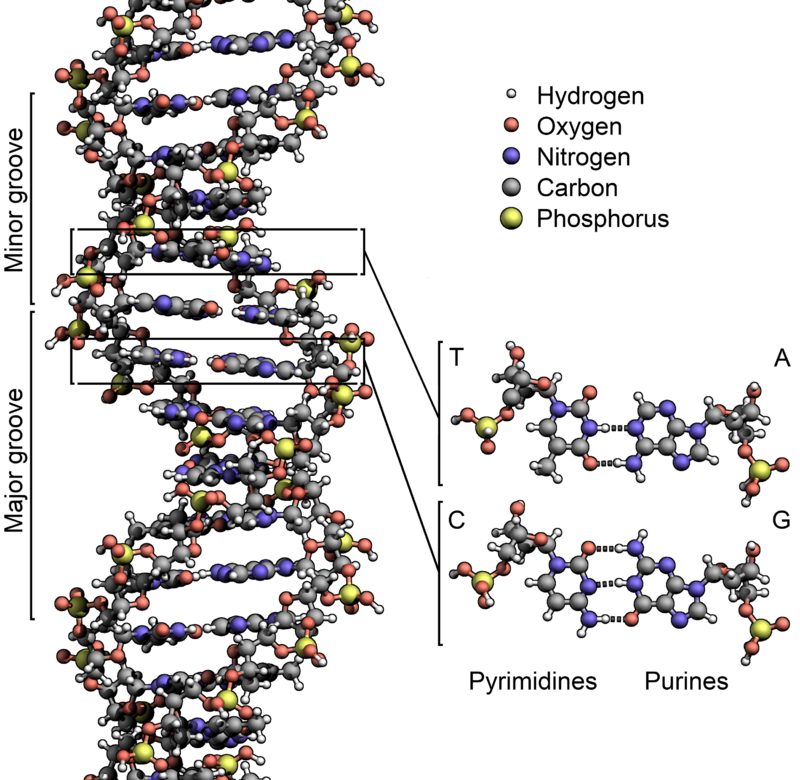
\includegraphics[width=0.7\textwidth]{c4.string.dna.00.png}
  \end{figure}
\end{frame}

\begin{frame}
  \frametitle{序列和字符串 | 序列表征 | 核酸}
  \begin{figure}
    \centering
    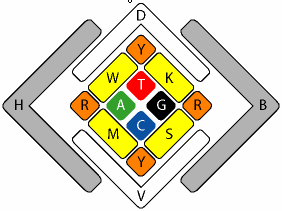
\includegraphics[width=0.85\textwidth]{c4.iub.base.01.png}
  \end{figure}
\end{frame}

\begin{frame}
  \frametitle{序列和字符串 | 序列表征 | 核酸}
  \begin{figure}
    \centering
    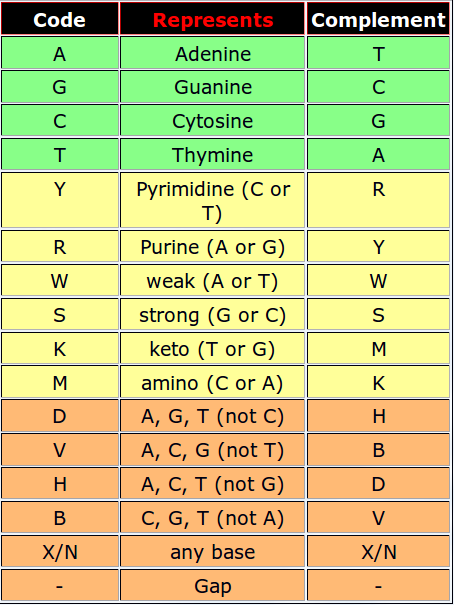
\includegraphics[width=0.7\textwidth,height=0.8\textheight]{c4.iub.base.02.png}
  \end{figure}
\end{frame}

\begin{frame}
  \frametitle{序列和字符串 | 序列表征 | 氨基酸}
  \begin{figure}
    \centering
    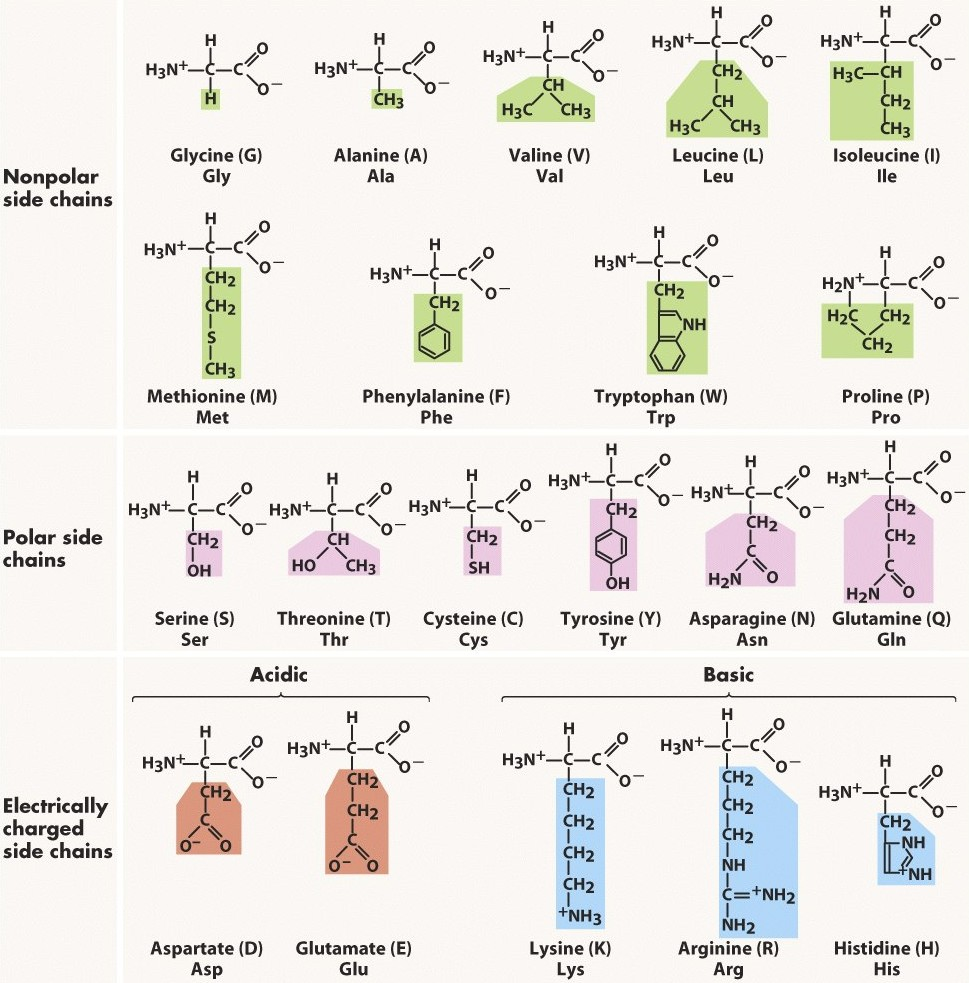
\includegraphics[width=0.8\textwidth,height=0.8\textheight]{c4.iub.aa.01.jpg}
  \end{figure}
\end{frame}

\begin{frame}
  \frametitle{序列和字符串 | 序列表征 | 字符串}
  \begin{block}{字符串}
    字符串(string),是由零个或多个字符组成的有限序列,是编程语言中表示文本的数据类型。
  \end{block}
  \pause
  \begin{block}{字符串操作}
    \begin{itemize}
      \item 通常以串的整体作为操作对象,如:在串中查找某个子串、求取一个子串、在串的某个位置上插入一个子串以及删除一个子串等。
      \item 两个字符串相等的充要条件是:长度相等,并且各个对应位置上的字符都相等。
      \item 设p、q是两个串,求q在p中首次出现的位置的运算叫做模式匹配。
      \item 一个简单的字符串操作是“拼接”:也就是说先写一个字符串S,随后在后面再写一个T得到ST这样一个过程。
      \item 其它的常见操作包括在一个长字符串中搜索一个子串,排列一组字符串以及分析一个字符串。
    \end{itemize}
  \end{block}
\end{frame}

\begin{frame}
  \frametitle{序列和字符串 | 序列表征 | 字符串}
  \begin{block}{序列与字符串\alert{(问题转换)}}
    生物信息学:(生物学)DNA/RNA/蛋白质序列 $\Longrightarrow$ 字符串(计算机科学)
  \end{block}
  \begin{figure}
    \centering
    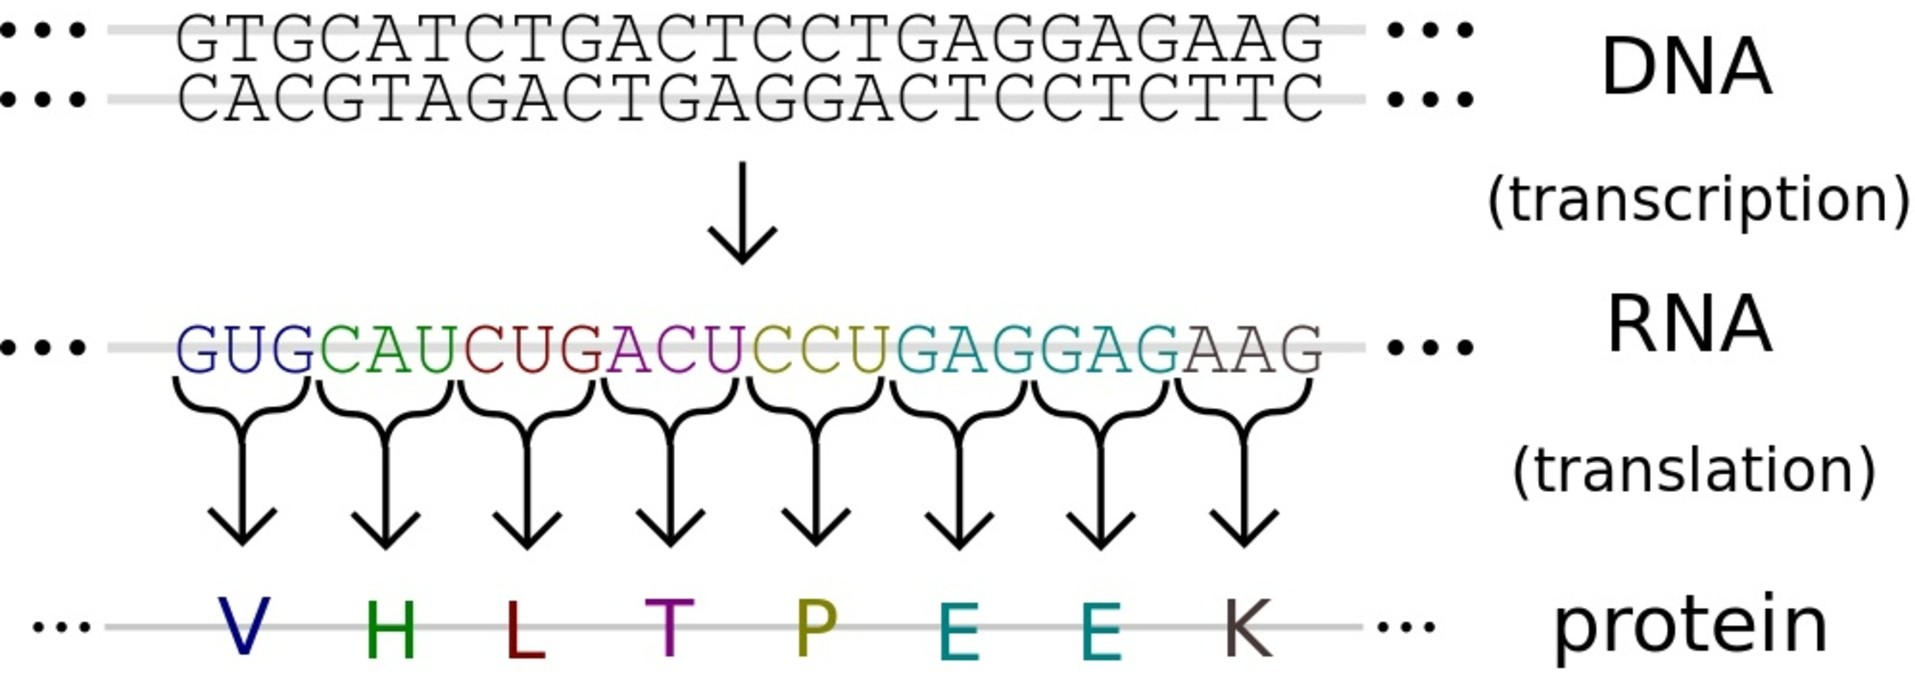
\includegraphics[width=0.9\textwidth]{c4.string.seq.01.jpg}
  \end{figure}
\end{frame}

\section{存储DNA序列}
\subsection{Perl程序}
\begin{frame}[fragile,label=exam4.1]
  \frametitle{序列和字符串 | 存储DNA | \alert{程序4.1}}
\begin{lstlisting}
#!/usr/bin/perl -w
# Example 4-1   Storing DNA in a variable, and printing it out

# First we store the DNA in a variable called $DNA
$DNA = 'ACGGGAGGACGGGAAAATTACTACGGCATTAGC';

# Next, we print the DNA onto the screen
print $DNA;

# Finally, we'll specifically tell the program to exit.
exit;
\end{lstlisting}
\end{frame}

\begin{frame}[fragile]
  \frametitle{序列和字符串 | 存储DNA | 程序 | \alert{补充}}
  \begin{itemize}
    \item 在Perl中,变量就是要处理的数据的名称,使用该名称,你可以对数据进行完全的访问。
    \item 变量起名要清晰易懂;既然是存储DNA序列,起名为 \verb|$DNA|再自然不过了(或者 \verb|$dna|、\verb|$dna_seq|……)。
    \item 保存程序时一定要保存为ASCII或者纯文本格式。
    \item 运行程序:\verb|perl example4-1.pl|(或者:\verb|chmod 755 example4-1.pl; ./example4-1.pl|)。
  \end{itemize}
\end{frame}

\subsection{控制流}
\begin{frame}
  \frametitle{序列和字符串 | 存储DNA | 控制流}
  所谓控制流,就是计算机是以什么顺序来执行程序中的语句的。\\
  \vspace{1em}
  所有的程序都是从第一行开始执行,除非明确指明了其他的运行顺序,否则它将一条一条地按照顺序执行语句,直到程序的最后一行。\\
  \vspace{1em}
  可以通过条件流程控制语句(if等)、循环流程控制语句(while等)等控制程序的执行顺序。
\end{frame}

\subsection{注释}
\begin{frame}[fragile]
  \frametitle{序列和字符串 | 存储DNA | 注释}
  \begin{itemize}
    \item 添加空行使程序更加易读。
    \item 以 \verb|#|起始进行注释。
    \item Perl程序运行时,会把空行和注释忽略掉。
    \item 注释内容:程序的用途、作者及相关信息,代码每一部分的作用,代码的工作原理,……
  \end{itemize}
  \pause
  \begin{block}{没有注释的、赤裸裸的、完全等价的程序}
\begin{lstlisting}
#!/usr/bin/perl -w
$DNA = 'ACGGGAGGACGGGAAAATTACTACGGCATTAGC';
print $DNA;
exit;
\end{lstlisting}
  \end{block}
\end{frame}

\subsection{命令解释}
\begin{frame}[fragile]
  \frametitle{序列和字符串 | 存储DNA | \alert{命令解释}}
\begin{lstlisting}
#!/usr/bin/perl -w
\end{lstlisting}
\pause
\begin{block}{命令解释}
  \begin{itemize}
    \item 像是注释,但并不是注释。
    \item 告诉Unix/Linux计算机,这是一个Perl程序。
    \item 本质上是Perl语言解释器在文件系统中的绝对路径。
    \item 标志 \verb|-w|,等同于 \verb|use warnings;|。使Perl在遇到错误时打印出相关信息。
    \item 注意:错误信息中的行号不一定准确,但是可以作为参考(通常错误就在对应行的附近)。
  \end{itemize}
\end{block}
\end{frame}

\begin{frame}[fragile]
  \frametitle{序列和字符串 | 存储DNA | 命令解释}
\begin{lstlisting}
#!/usr/bin/perl
#!/usr/bin/env perl
#!/usr/local/bin/perl
#!/bin/perl
...
\end{lstlisting}
\end{frame}

\subsection{语句}
\begin{frame}[fragile]
  \frametitle{序列和字符串 | 存储DNA | \alert{语句}}
\begin{lstlisting}
$DNA = 'ACGGGAGGACGGGAAAATTACTACGGCATTAGC';
\end{lstlisting}
\pause
\begin{block}{语句}
  \begin{itemize}
    \item 这行代码在Perl语言中叫做语句(statement)。
    \item 在Perl中,语句以分号 \verb|;|结尾(类似于英语中以句号 \verb|.|进行结尾)。
    \item 该行是一个赋值语句:把DNA序列存储到 \verb|$DNA|变量中。
  \end{itemize}
\end{block}
\end{frame}

\begin{frame}
  \frametitle{序列和字符串 | 存储DNA | 语句 | 断句}
  \begin{figure}
    \centering
    
\includegraphics[width=0.48\textwidth]{c4.string.statement.01.jpg}
    \quad
    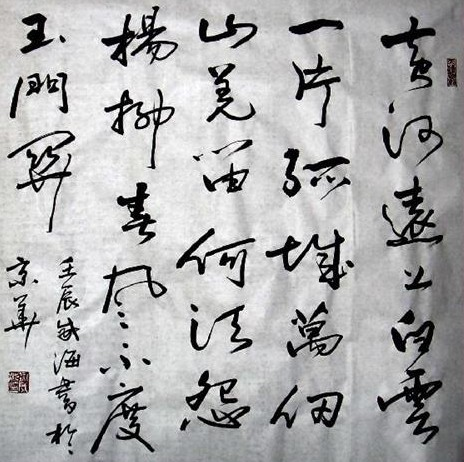
\includegraphics[width=0.44\textwidth]{c4.string.statement.02.jpg}
  \end{figure}
\end{frame}

\begin{frame}
  \frametitle{序列和字符串 | 存储DNA | 变量}
  \begin{figure}
    \centering
    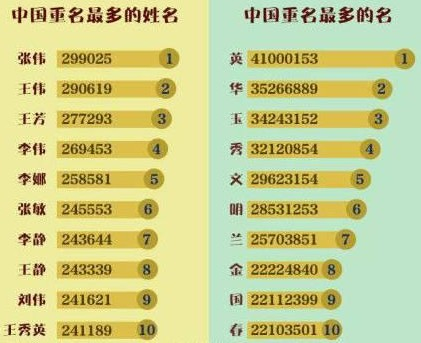
\includegraphics[width=0.54\textwidth]{c4.string.name.01.jpg}
    \quad
    
\includegraphics[width=0.4\textwidth]{c4.string.name.02.jpg}
  \end{figure}
\end{frame}

\begin{frame}[fragile]
  \frametitle{序列和字符串 | 存储DNA | \alert{变量}}
  \begin{block}{变量名}
  \begin{itemize}
    \item Perl中变量名的规范:只能由大小写字母、数字和下划线 \verb|_|组成,且第一个字符不能是数字。
    \item 只要合法,什么样的变量名对于计算机来说都无所谓,都是一样的。
    \item 有意义的变量名可以清晰地表明程序中变量的作用,使程序易读、易理解。
    \item 精心选择有意义的变量名是一个好习惯。
  \end{itemize}
  \end{block}
  \pause
  \begin{block}{标量变量}
    \begin{itemize}
      \item 标量变量(scalar variable):存储单个数据项目的变量,在Perl中以美元符号 \verb|$|起始。
      \item 一个标量变量一次只能存储数据中的一个项目。
      \item 使用标量变量存储字符串或者数字(比如:hello,25、6.234、3.5E10、-0.8373)。
    \end{itemize}
  \end{block}
\end{frame}

\begin{frame}[fragile]
  \frametitle{序列和字符串 | 存储DNA | 变量 | perlstyle}
  \begin{block}{变量}
    \begin{itemize}
      \item {\small 
Perl语言从C那里继承了一部分命名约定。局部变量与子例程通常使用用下划线分隔开的小写单词来命名;如果是私有变量或子例程,则在前面加一个下划线以表明其私有性;Perl包中的变量命名则采用单词首字母大写的方式(像英文标题那样);如果是声明的常量,需要全部大写;Perl包的名字,除了pragmata(如strict),则一律采用“CamelCase”的方式。}
      \item \href{https://en.wikipedia.org/wiki/Naming\_convention\_(programming)}{Naming convention (programming)}
    \end{itemize}
  \end{block}
  \pause
  \vspace{-0.5em}
  \begin{block}{缩进与大括号}
    \begin{itemize}
      \item K\&R style, Allman style, Whitesmiths style, GNU style
      \item \href{http://catb.org/jargon/html/I/indent-style.html}{indent style}
    \end{itemize}
  \end{block}
  \pause
  \vspace{-0.5em}
  \begin{block}{perlstyle}
    \begin{itemize}
      \item \verb|perldoc perlstyle|
      \item \href{http://perldoc.perl.org/perlstyle.html}{perlstyle - Perl style guide}
    \end{itemize}
  \end{block}
\end{frame}

\begin{frame}[fragile]
  \frametitle{序列和字符串 | 存储DNA | \alert{字符串}}
  \begin{block}{字符串}
    \begin{itemize}
      \item 在Perl中,把序列等放在引号(单引号或者双引号)中表明它是字符串。
      \item 单引号(\verb|' '|)不会进行变量内插。
      \item 双引号(\verb|" "|)能够进行变量内插,可以使用转义字符。
    \end{itemize}
  \end{block}
  \pause
\begin{lstlisting}
# 此处两者完全等价
$DNA = 'ACGGGAGGACGGGAAAATTACTACGGCATTAGC';
$DNA = "ACGGGAGGACGGGAAAATTACTACGGCATTAGC";

# 此处结果完全不同(变量内插)
print '$DNA';
print "$DNA";
\end{lstlisting}
\end{frame}

\begin{frame}[fragile]
  \frametitle{序列和字符串 | 存储DNA | \alert{赋值}}
  \begin{block}{赋值}
    \begin{itemize}
      \item 使用等号 \verb|=|来把一个变量设成特定的值。
      \item \verb|=|叫做赋值操作符(assignment operator)。
      \item 赋值后就可以通过变量名来获取它的值了。
      \item 注意赋值语句中项目的顺序:变量在左边(lvalue),要赋给变量的值在右边(rvalue)。
      \item 牢记在Perl中 \verb|=|不表示相等(数学),而是进行赋值。
    \end{itemize}
  \end{block}
\end{frame}

\begin{frame}[fragile]
  \frametitle{序列和字符串 | 存储DNA | 打印输出}
  \begin{block}{打印输出}
    \begin{itemize}
      \item 使用 \verb|print|函数,它会把变量的值直接打印输出出来。
      \item \verb|print|处理的是标量变量。
      \item 默认是输出到计算机屏幕(标准输出设备, STDOUT)上。
    \end{itemize}
  \end{block}
  \pause
\begin{lstlisting}
# 两者效果相同
print $DNA;
print "$DNA";

# 不会输出序列
print '$DNA';
\end{lstlisting}
\end{frame}

\begin{frame}[fragile]
  \frametitle{序列和字符串 | 存储DNA | \alert{退出}}
  \begin{block}{退出}
    \begin{itemize}
      \item 使用 \verb|exit;|语句明确告诉计算机退出程序。
      \item 在Perl中,程序末尾的 \verb|exit;|并不是必需的。
      \item Perl程序一旦运行到末尾,就会自动退出。
    \end{itemize}
  \end{block}
\end{frame}

\begin{frame}[fragile]
  \frametitle{序列和字符串 | 存储DNA | 程序4.1}
\begin{lstlisting}
#!/usr/bin/perl -w

$DNA = 'ACGGGAGGACGGGAAAATTACTACGGCATTAGC';

print $DNA;

exit;
\end{lstlisting}
\end{frame}

%\againframe{exam4.1}

\section{拼接DNA片段}
\begin{frame}
  \frametitle{序列和字符串 | 拼接DNA}
  \begin{block}{拼接(concatenate)}
    \begin{itemize}
      \item 把一个字符串附加到另一个字符串的末尾。
      \item 把AT和GC拼接起来,得到ATGC。
    \end{itemize}
  \end{block}
  \pause
  \begin{block}{生物学中的应用}
    \begin{itemize}
      \item 把克隆插入到细胞载体中
      \item 把剪切后的外显子拼接起来(“剪接”中的“接”)
      \item ……
    \end{itemize}
  \end{block}
\end{frame}

\begin{frame}[fragile,label=exam4.2.1]
  \frametitle{序列和字符串 | 拼接DNA | 程序4.2.1}
\begin{lstlisting}
#!/usr/bin/perl -w
# Example 4-2   Concatenating DNA

# Store two DNA fragments into two variables called $DNA1 and $DNA2
$DNA1 = 'ACGGGAGGACGGGAAAATTACTACGGCATTAGC';
$DNA2 = 'ATAGTGCCGTGAGAGTGATGTAGTA';

# Print the DNA onto the screen
print "Here are the original two DNA fragments:\n\n";

print $DNA1, "\n";

print $DNA2, "\n\n";
\end{lstlisting}
\end{frame}

\begin{frame}[fragile,label=exam4.2.2]
  \frametitle{序列和字符串 | 拼接DNA | 程序4.2.2}
\begin{lstlisting}[firstnumber=15]
# Concatenate the DNA fragments into a third variable and print them
# Using "string interpolation"
$DNA3 = "$DNA1$DNA2";

print "Here is the concatenation of the first two fragments (version 1):\n\n";

print "$DNA3\n\n";
\end{lstlisting}
\end{frame}

\begin{frame}[fragile,label=exam4.2.3]
  \frametitle{序列和字符串 | 拼接DNA | 程序4.2.3}
\begin{lstlisting}[firstnumber=23]
# An alternative way using the "dot operator":
# Concatenate the DNA fragments into a third variable and print them
$DNA3 = $DNA1 . $DNA2;

print "Here is the concatenation of the first two fragments (version 2):\n\n";

print "$DNA3\n\n";
\end{lstlisting}
\end{frame}

\begin{frame}[fragile,label=exam4.2.4]
  \frametitle{序列和字符串 | 拼接DNA | 程序4.2.4}
\begin{lstlisting}[firstnumber=31]
# Print the same thing without using the variable $DNA3
print "Here is the concatenation of the first two fragments (version 3):\n\n";

print $DNA1, $DNA2, "\n";

exit;
\end{lstlisting}
\end{frame}

\begin{frame}[fragile]
  \frametitle{序列和字符串 | 拼接DNA | 程序4.2 | 输出}
\begin{lstlisting}[language=,basicstyle=\scriptsize\tt,numberstyle=\scriptsize]
Here are the original two DNA fragments:

ACGGGAGGACGGGAAAATTACTACGGCATTAGC
ATAGTGCCGTGAGAGTGATGTAGTA

Here is the concatenation of the first two fragments (version 1):

ACGGGAGGACGGGAAAATTACTACGGCATTAGCATAGTGCCGTGAGAGTGATGTAGTA

Here is the concatenation of the first two fragments (version 2):

ACGGGAGGACGGGAAAATTACTACGGCATTAGCATAGTGCCGTGAGAGTGATGTAGTA

Here is the concatenation of the first two fragments (version 3):

ACGGGAGGACGGGAAAATTACTACGGCATTAGCATAGTGCCGTGAGAGTGATGTAGTA
\end{lstlisting}
\end{frame}

\begin{frame}[fragile]
  \frametitle{序列和字符串 | 拼接DNA | \alert{print语句}}
\begin{lstlisting}
print $DNA1, "\n";
print $DNA2, "\n\n";
\end{lstlisting}
\pause
\begin{block}{说明}
  \begin{itemize}
    \item \verb|\n|:换行符,定位到下一行的开头
    \item \verb|\n\n|:两个新行(中间添加一个空行)
    \item 空行:没有任何打印输出的行(取决于操作系统)
    \item 包裹在双引号中的换行符表示它们是字符串的一部分
    \item \verb|"\n"|会输出换行符,\verb|'\n'|输出 \verb|\n|本身
    \item 逗号分隔列表中的项目,print语句会输出列表中的所有项目
  \end{itemize}
\end{block}
\end{frame}

\begin{frame}[fragile]
  \frametitle{序列和字符串 | 拼接DNA | \alert{拼接语句}}
\begin{lstlisting}
$DNA3 = "$DNA1$DNA2"; print "$DNA3\n\n";
$DNA3 = $DNA1 . $DNA2; print "$DNA3\n\n";
print $DNA1, $DNA2, "\n";
print "$DNA1$DNA2\n";
...
\end{lstlisting}
\begin{block}{说明}
\begin{itemize}
  \item 字符串内插(string interpolation)/变量替换:双引号会把字符串中的变量替换成变量的值(必要时可以使用大括号来保护变量)
  \item 点操作符:拼接字符串
  \item 使用print语句
  \item There's more than one way to do it.
  \item There are more than two ways to do it.
\end{itemize}
\end{block}
\end{frame}

\begin{frame}[fragile]
  \frametitle{序列和字符串 | 拼接DNA | 标量变量}
  \begin{block}{标量变量}
    \begin{itemize}
      \item 标量变量可以存储字符串、整数、浮点数、布尔值等
      \item Perl能够“智能”判断存储的是哪种类型的数据
    \end{itemize}
  \end{block}
  \pause
\begin{lstlisting}
$number = 17;
print $number, "\n";
\end{lstlisting}
\end{frame}

\begin{frame}[fragile]
  \frametitle{序列和字符串 | 拼接DNA | \alert{程序4.2}}
\begin{lstlisting}[basicstyle=\small\tt]
#!/usr/bin/perl -w

$DNA1 = 'ACGGGAGGACGGGAAAATTACTACGGCATTAGC';
$DNA2 = 'ATAGTGCCGTGAGAGTGATGTAGTA';

print $DNA1, "\n";
print $DNA2, "\n\n";

$DNA3 = "$DNA1$DNA2";
print "$DNA3\n\n";

$DNA3 = $DNA1 . $DNA2;
print "$DNA3\n\n";

print $DNA1, $DNA2, "\n";

exit;
\end{lstlisting}
\end{frame}

\section{DNA转录成RNA}
\begin{frame}
  \frametitle{序列和字符串 | 转录}
  \begin{figure}
    \centering
    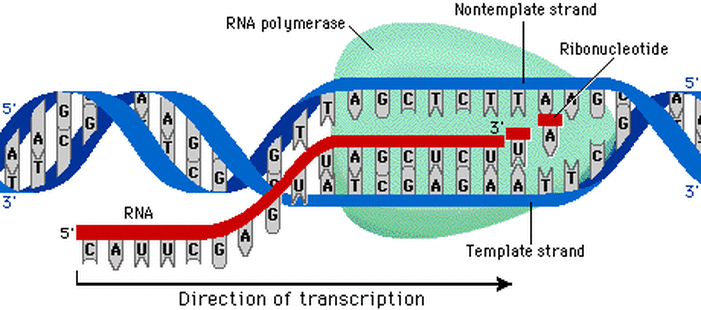
\includegraphics[width=0.9\textwidth]{c4.string.transcription.01.png}
  \end{figure}
  \pause
  \begin{block}{问题简化}
    DNA转录成RNA $\Longrightarrow$ 把DNA中所有的T替换成U
  \end{block}
\end{frame}

\begin{frame}[fragile,label=exam4.3.1]
  \frametitle{序列和字符串 | 转录 | 程序4.3.1}
\begin{lstlisting}
#!/usr/bin/perl -w
# Example 4-3   Transcribing DNA into RNA

# The DNA
$DNA = 'ACGGGAGGACGGGAAAATTACTACGGCATTAGC';

# Print the DNA onto the screen
print "Here is the starting DNA:\n\n";

print "$DNA\n\n";
\end{lstlisting}
\end{frame}

\begin{frame}[fragile,label=exam4.3.2]
  \frametitle{序列和字符串 | 转录 | 程序4.3.2}
\begin{lstlisting}[firstnumber=12]
# Transcribe the DNA to RNA by substituting all T's with U's.
$RNA = $DNA;

$RNA =~ s/T/U/g;

# Print the RNA onto the screen
print "Here is the result of transcribing the DNA to RNA:\n\n";

print "$RNA\n";

# Exit the program.
exit;
\end{lstlisting}
\end{frame}

\begin{frame}[fragile]
  \frametitle{序列和字符串 | 转录 | 程序4.3 | 输出}
\begin{lstlisting}[language=]
Here is the starting DNA:

ACGGGAGGACGGGAAAATTACTACGGCATTAGC

Here is the result of transcribing the DNA to RNA:

ACGGGAGGACGGGAAAAUUACUACGGCAUUAGC
\end{lstlisting}
\end{frame}

\begin{frame}
  \frametitle{序列和字符串 | 转录| Perl特性}
  \begin{itemize}
    \item Perl能够轻松处理DNA字符串等文本数据
    \item 常见操作:翻译、反转、替换、删除、排序等
    \item Perl在生物信息学领域独领风骚的主要原因(之一)
  \end{itemize}
\end{frame}

\begin{frame}[fragile]
  \frametitle{序列和字符串 | 转录 | \alert{语句}}
\begin{lstlisting}
# $RNA开始存储的其实是DNA
$RNA = $DNA;
# 替换后,$RNA存储的才是RNA
$RNA =~ s/T/U/g;

# 完全等价的语句
# $RNA存储的就真的只是RNA了
($RNA = $DNA) =~ s/T/U/g;
\end{lstlisting}
\end{frame}

\begin{frame}
  \frametitle{序列和字符串 | 转录 | \alert{绑定操作符和替换}}
  \begin{figure}
    \centering
    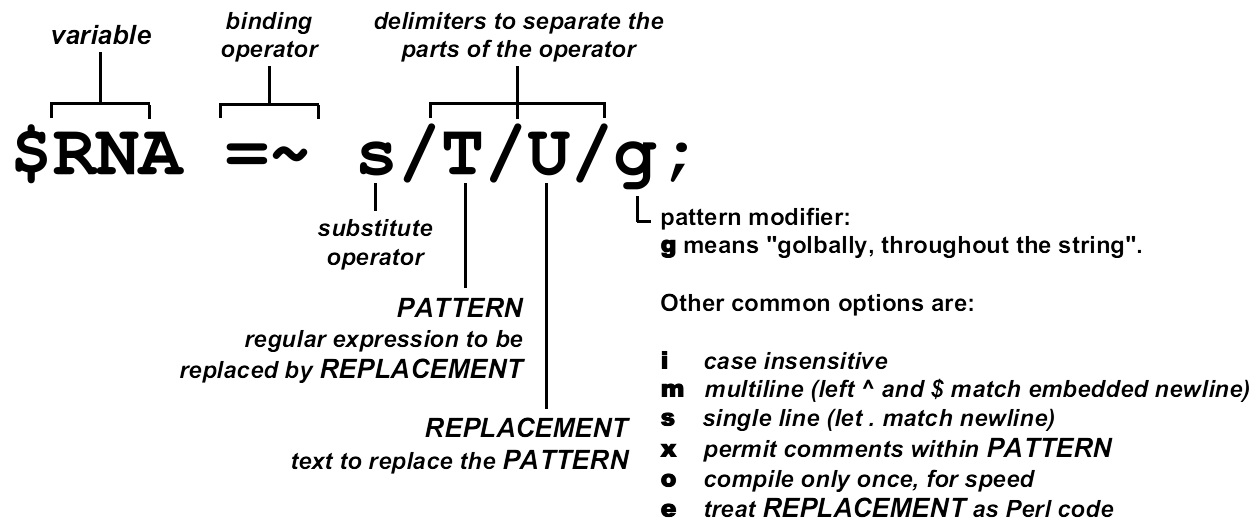
\includegraphics[width=\textwidth]{c4.string.sub.png}
  \end{figure}
\end{frame}

\begin{frame}[fragile]
  \frametitle{序列和字符串 | 转录 | \alert{程序4.3}}
\begin{lstlisting}
#!/usr/bin/perl -w

$DNA = 'ACGGGAGGACGGGAAAATTACTACGGCATTAGC';

print "Here is the starting DNA:\n\n";
print "$DNA\n\n";

$RNA = $DNA;
$RNA =~ s/T/U/g;

print "Here is the result of transcribing the DNA to RNA:\n\n";
print "$RNA\n";

exit;
\end{lstlisting}
\end{frame}


\section{使用Perl文档}
\begin{frame}[fragile]
  \frametitle{序列和字符串 | \alert{Perl文档}}
  \begin{itemize}
    \item \href{http://www.perl.com/}{http://www.perl.com/} 
    \item \verb|perldoc -f print|(perldoc手册:\verb|man perldoc|)
    \item 文档太全,直接忽略掉对你来说毫无意义的内容吧
    \item 翻阅文档是学习Perl的绝佳途径(不要“骑着驴找驴”)
  \end{itemize}
\end{frame}

\section{序列反向互补}
\begin{frame}
  \frametitle{序列和字符串 | 反向互补}
  \begin{block}{应用}
    \begin{itemize}
      \item 给出一条链,输出另一条链
      \item 在查询DNA时,自动查询其反向互补序列
      \item 从基因的负链得到正链
      \item ……
    \end{itemize}
  \end{block}
\end{frame}

\begin{frame}[fragile]
  \frametitle{序列和字符串 | 反向互补 | 程序4.4.1}
\begin{lstlisting}
#!/usr/bin/perl -w
# Example 4-4   Calculating the reverse complement of a strand of DNA

# The DNA
$DNA = 'ACGGGAGGACGGGAAAATTACTACGGCATTAGC';

# Print the DNA onto the screen
print "Here is the starting DNA:\n\n";

print "$DNA\n\n";
\end{lstlisting}
\end{frame}

\begin{frame}[fragile]
  \frametitle{序列和字符串 | 反向互补 | 程序4.4.2}
\begin{lstlisting}[firstnumber=12,basicstyle=\footnotesize\tt]
# Calculate the reverse complement
#  Warning: this attempt will fail!
#
# First, copy the DNA into new variable $revcom
# (short for REVerse COMplement)
# Notice that variable names can use lowercase letters like
# "revcom" as well as uppercase like "DNA".  In fact,
# lowercase is more common.
#
# It doesn't matter if we first reverse the string and then
# do the complementation; or if we first do the complementation
# and then reverse the string.  Same result each time.
# So when we make the copy we'll do the reverse in the same statement.
\end{lstlisting}
\end{frame}

\begin{frame}[fragile]
  \frametitle{序列和字符串 | 反向互补 | 程序4.4.3}
\begin{lstlisting}[firstnumber=27,basicstyle=\footnotesize\tt]
$revcom = reverse $DNA;

#
# Next substitute all bases by their complements,
# A->T, T->A, G->C, C->G
#

$revcom =~ s/A/T/g;
$revcom =~ s/T/A/g;
$revcom =~ s/G/C/g;
$revcom =~ s/C/G/g;

# Print the reverse complement DNA onto the screen
print "Here is the reverse complement DNA:\n\n";

print "$revcom\n";
\end{lstlisting}
\end{frame}

\begin{frame}[fragile]
  \frametitle{序列和字符串 | 反向互补 | 程序4.4.4}
\begin{lstlisting}[firstnumber=45,basicstyle=\scriptsize\tt]
# Oh-oh, that didn't work right!
# Our reverse complement should have all the bases in it, since the
# original DNA had all the bases-but ours only has A and G!
#
# Do you see why?
#
# The problem is that the first two substitute commands above change
# all the A's to T's (so there are no A's) and then all the
# T's to A's (so all the original A's and T's are all now A's).
# Same thing happens to the G's and C's all turning into G's.
#

print "\nThat was a bad algorithm, and the reverse complement was wrong!\n";
print "Try again ... \n\n";
\end{lstlisting}
\end{frame}

\begin{frame}[fragile]
  \frametitle{序列和字符串 | 反向互补 | 程序4.4.5}
\begin{lstlisting}[firstnumber=60,basicstyle=\small\tt]
# Make a new copy of the DNA (see why we saved the original?)
$revcom = reverse $DNA;

# See the text for a discussion of tr///
$revcom =~ tr/ACGTacgt/TGCAtgca/;

# Print the reverse complement DNA onto the screen
print "Here is the reverse complement DNA:\n\n";

print "$revcom\n";

print "\nThis time it worked!\n\n";

exit;
\end{lstlisting}
\end{frame}

\begin{frame}[fragile]
  \frametitle{序列和字符串 | 反向互补 | 程序4.4.1 | 输出}
\begin{lstlisting}[language=,basicstyle=\small\tt]
Here is the starting DNA:

ACGGGAGGACGGGAAAATTACTACGGCATTAGC

Here is the reverse complement DNA:

GGAAAAGGGGAAGAAAAAAAGGGGAGGAGGGGA

That was a bad algorithm, and the reverse complement was wrong!
Try again ...

Here is the reverse complement DNA:

GCTAATGCCGTAGTAATTTTCCCGTCCTCCCGT

This time it worked!
\end{lstlisting}
\end{frame}

\begin{frame}
  \frametitle{序列和字符串 | 反向互补}
   \begin{block}{相似的经历}
     \begin{enumerate}
       \item 编写代码
       \item 代码不工作
       \item 解决问题(修正语法,重新思考、设计新的方法,……)
     \end{enumerate}
   \end{block} 
   \pause
   \begin{block}{解决策略}
     \begin{itemize}
       \item 检查代码的细节
       \item 查阅文档
       \item 检索(特性,模块,……)
     \end{itemize}
   \end{block}
\end{frame}

\begin{frame}
  \frametitle{序列和字符串 | 反向互补 | \alert{tr}}
  \begin{itemize}
    \item reverse函数:反转字符串等元素的顺序
    \item tr函数:一次性把一个字符集翻译成新的字符
  \end{itemize}
  \begin{figure}
    \centering
    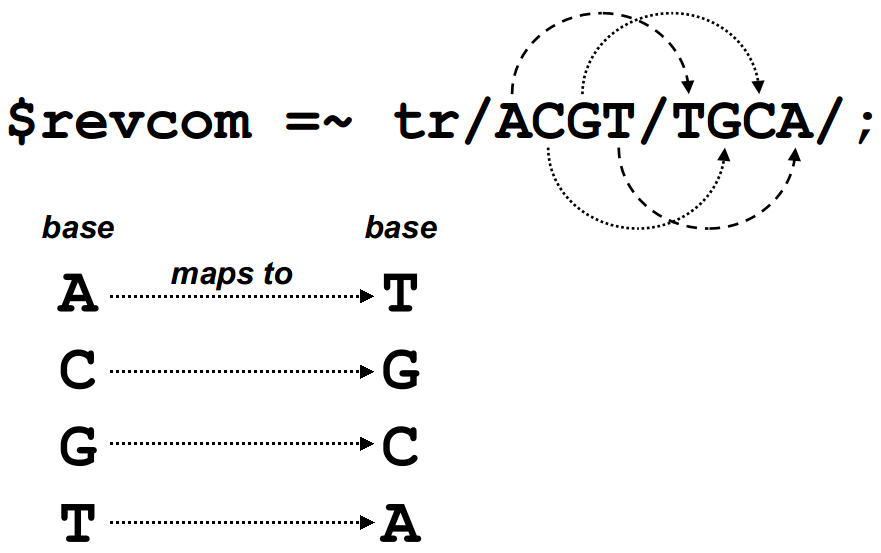
\includegraphics[width=0.7\textwidth]{c4.string.tr.png}
  \end{figure}
\end{frame}

\begin{frame}[fragile]
  \frametitle{序列和字符串 | 反向互补 | \alert{程序4.4}}
\begin{lstlisting}
#!/usr/bin/perl -w

$DNA = 'ACGGGAGGACGGGAAAATTACTACGGCATTAGC';

print "Here is the starting DNA:\n\n";
print "$DNA\n\n";

$revcom = reverse $DNA;
$revcom =~ tr/ACGTacgt/TGCAtgca/;

print "Here is the reverse complement DNA:\n\n";
print "$revcom\n";

exit;
\end{lstlisting}
\end{frame}

\begin{frame}
  \frametitle{序列和字符串 | 小结}
  \begin{block}{已经学习}
    \begin{itemize}
      \item 存储DNA序列
      \item 把DNA片段拼接起来
      \item 把DNA转录成RNA
      \item 获取反向互补序列
    \end{itemize}
  \end{block}
  \pause
  \begin{block}{即将学习}
    \begin{itemize}
      \item 在Perl中使用蛋白质序列数据
      \item 从文件读取蛋白质序列数据
      \item Perl语言中的数组
      \item Perl语言中的上下文
    \end{itemize}
  \end{block}
\end{frame}

\section{从文件读取数据}
\begin{frame}[fragile]
  \frametitle{序列和字符串 | 读取文件 | 创建数据}
\begin{lstlisting}[language=,xrightmargin=1em,basicstyle=\footnotesize\tt,numberstyle=\scriptsize]
MNIDDKLEGLFLKCGGIDEMQSSRTMVVMGGVSGQSTVSGELQD
SVLQDRSMPHQEILAADEVLQESEMRQQDMISHDELMVHEETVKNDEEQMETHERLPQ
GLQYALNVPISVKQEITFTDVSEQLMRDKKQIR
\end{lstlisting}
\pause
\begin{block}{补充说明}
  \begin{itemize}
    \item 认真组织文件和文件夹
    \item 仔细考虑文件和文件夹的命名
    \item 尽量仅通过文件名、而不需要打开文件就可以对文件保存的数据有所了解
    \item 比如:\verb|NM_021964fragment.pep|
  \end{itemize}
\end{block}
\end{frame}

\begin{frame}[fragile]
  \frametitle{序列和字符串 | 读取文件 | 程序4.5.1}
\begin{lstlisting}
#!/usr/bin/perl -w
# Example 4-5   Reading protein sequence data from a file

# The filename of the file containing the protein sequence data
$proteinfilename = 'NM_021964fragment.pep';

# First we have to "open" the file, and associate
# a "filehandle" with it.  We choose the filehandle
# PROTEINFILE for readability.
\end{lstlisting}  
\end{frame}

\begin{frame}[fragile]
  \frametitle{序列和字符串 | 读取文件 | 程序4.5.2}
\begin{lstlisting}[firstnumber=10,basicstyle=\footnotesize\tt]
open( PROTEINFILE, $proteinfilename );

# Now we do the actual reading of the protein sequence data from the file,
# by using the angle brackets < and > to get the input from the
# filehandle.  We store the data into our variable $protein.
$protein = <PROTEINFILE>;

# Now that we've got our data, we can close the file.
close PROTEINFILE;

# Print the protein onto the screen
print "Here is the protein:\n\n";

print $protein;

exit;
\end{lstlisting}  
\end{frame}

\begin{frame}[fragile]
  \frametitle{序列和字符串 | 读取文件 | 程序4.5 | 输出}
\begin{lstlisting}[language=]
Here is the protein:

MNIDDKLEGLFLKCGGIDEMQSSRTMVVMGGVSGQSTVSGELQD
\end{lstlisting}
\end{frame}

\begin{frame}[fragile]
  \frametitle{序列和字符串 | 读取文件 | \alert{处理方法}}
\begin{lstlisting}
# 第一步: 把文件和文件句柄关联起来,之后对文件的操作都通过文件句柄来进行
open( PROTEINFILE, $proteinfilename );
# 第二步:读取文件中的数据
$protein = <PROTEINFILE>;
# 第三步:把文件和文件句柄解关联
close PROTEINFILE;
\end{lstlisting}
\pause
\begin{block}{补充说明}
  \begin{itemize}
    \item open函数还有很多选项,用于精确指定如何使用文件
    \item 文件句柄通常使用大写字母
    \item \verb|< >|:输入操作符,从文件中读取数据
    \item 好习惯:有open就有close
  \end{itemize}
\end{block}
\end{frame}

\begin{frame}[fragile]
  \frametitle{序列和字符串 | 读取文件 | \alert{处理方法}}
\begin{lstlisting}[basicstyle=\small\tt]
# 读取文件
open my $FH, '<', $filename or die "$0 : failed to open input file '$filename' : $!\n";
... <$FH> ...
close $FH or warn "$0 : failed to close input file '$filename' : $!\n";

# 写入文件
open my $FH_OUT, '>', $fn_out or die "$0 : failed to open output file '$fn_out' : $!\n";
select $FH_OUT;
# OR: use $FH_OUT for every print
print $FH_OUT "something...";
... 
close $FH_OUT or warn "$0 : failed to close output file '$fn_out' : $!\n";
\end{lstlisting}
\end{frame}

\begin{frame}[fragile]
  \frametitle{序列和字符串 | 读取文件 | 程序4.6.1}
\begin{lstlisting}
#!/usr/bin/perl -w
# Example 4-6   Reading protein sequence data from a file, take 2

# The filename of the file containing the protein sequence data
$proteinfilename = 'NM_021964fragment.pep';

# First we have to "open" the file, and associate
# a "filehandle" with it.  We choose the filehandle
# PROTEINFILE for readability.
open( PROTEINFILE, $proteinfilename );
\end{lstlisting}
\end{frame}

\begin{frame}[fragile]
  \frametitle{序列和字符串 | 读取文件 | 程序4.6.2}
\begin{lstlisting}[firstnumber=12]
# Now we do the actual reading of the protein sequence data from the file,
# by using the angle brackets < and > to get the input from the
# filehandle.  We store the data into our variable $protein.
#
# Since the file has three lines, and since the read only is
# returning one line, we'll read a line and print it, three times.
\end{lstlisting}
\end{frame}

\begin{frame}[fragile]
  \frametitle{序列和字符串 | 读取文件 | 程序4.6.3}
\begin{lstlisting}[firstnumber=19,basicstyle=\small\tt]
# First line
$protein = <PROTEINFILE>;

# Print the protein onto the screen
print "\nHere is the first line of the protein file:\n\n";

print $protein;

# Second line
$protein = <PROTEINFILE>;

# Print the protein onto the screen
print "\nHere is the second line of the protein file:\n\n";

print $protein;
\end{lstlisting}
\end{frame}

\begin{frame}[fragile]
  \frametitle{序列和字符串 | 读取文件 | 程序4.6.4}
\begin{lstlisting}[firstnumber=35]
# Third line
$protein = <PROTEINFILE>;

# Print the protein onto the screen
print "\nHere is the third line of the protein file:\n\n";

print $protein;

# Now that we've got our data, we can close the file.
close PROTEINFILE;

exit;
\end{lstlisting}
\end{frame}

\begin{frame}[fragile]
  \frametitle{序列和字符串 | 读取文件 | 程序4.6 | 输出}
\begin{lstlisting}[language=,basicstyle=\footnotesize\tt,xrightmargin=1em]
Here is the first line of the protein file:

MNIDDKLEGLFLKCGGIDEMQSSRTMVVMGGVSGQSTVSGELQD

Here is the second line of the protein file:

SVLQDRSMPHQEILAADEVLQESEMRQQDMISHDELMVHEETVKNDEEQMETHERLPQ

Here is the third line of the protein file:

GLQYALNVPISVKQEITFTDVSEQLMRDKKQIR
\end{lstlisting}
\end{frame}

\begin{frame}[fragile]
  \frametitle{序列和字符串 | 读取文件| \alert{程序4.6}}
\begin{lstlisting}[basicstyle=\small\tt]
#!/usr/bin/perl -w

$proteinfilename = 'NM_021964fragment.pep';

open( PROTEINFILE, $proteinfilename );

$protein = <PROTEINFILE>;
print $protein;
$protein = <PROTEINFILE>;
print $protein;
$protein = <PROTEINFILE>;
print $protein;

close PROTEINFILE;

exit;
\end{lstlisting}
\end{frame}

\begin{frame}[fragile]
  \frametitle{序列和字符串 | 读取文件| 程序4.6 | WRONG!}
\begin{lstlisting}[basicstyle=\small\tt]
#!/usr/bin/perl -w

$proteinfilename = 'NM_021964fragment.pep';

open( PROTEINFILE, $proteinfilename );

$protein = <PROTEINFILE>;
$protein = <PROTEINFILE>;
$protein = <PROTEINFILE>;
print $protein;
# What is wrong?

close PROTEINFILE;

exit;
\end{lstlisting}
\end{frame}

\begin{frame}[fragile]
  \frametitle{序列和字符串 | 读取文件 | 程序4.6 | 总结}
  \begin{block}{便捷之处}
    \begin{itemize}
      \item 自动读取文件的下一行
      \item 程序记录读取到哪儿,需要读取哪一行
    \end{itemize}
  \end{block}
  \pause
  \begin{block}{繁琐之处}
    \begin{itemize}
      \item 一次只能读取输入文件的一行
      \item 如果一个文件有成千上万行怎么办?
      \item 解决办法
        \begin{itemize}
          \item 数组
          \item 循环
        \end{itemize}
    \end{itemize}
  \end{block}
\end{frame}

\section{数组}
\subsection{Perl程序}
\begin{frame}[fragile]
  \frametitle{序列和字符串 | 数组 | 程序4.7.1}
\begin{lstlisting}
#!/usr/bin/perl -w
# Example 4-7   Reading protein sequence data from a file, take 3

# The filename of the file containing the protein sequence data
$proteinfilename = 'NM_021964fragment.pep';

# First we have to "open" the file
open( PROTEINFILE, $proteinfilename );
\end{lstlisting}
\end{frame}

\begin{frame}[fragile]
  \frametitle{序列和字符串 | 数组 | 程序4.7.2}
\begin{lstlisting}[firstnumber=10]
# Read the protein sequence data from the file, and store it
# into the array variable @protein
@protein = <PROTEINFILE>;

# Print the protein onto the screen
print @protein;

# Close the file.
close PROTEINFILE;

exit;
\end{lstlisting}
\end{frame}

\begin{frame}[fragile]
  \frametitle{序列和字符串 | 数组 | 程序4.7 | 输出}
\begin{lstlisting}[language=,basicstyle=\footnotesize\tt,xrightmargin=1em]
MNIDDKLEGLFLKCGGIDEMQSSRTMVVMGGVSGQSTVSGELQD
SVLQDRSMPHQEILAADEVLQESEMRQQDMISHDELMVHEETVKNDEEQMETHERLPQ
GLQYALNVPISVKQEITFTDVSEQLMRDKKQIR
\end{lstlisting}
\end{frame}

\begin{frame}[fragile]
  \frametitle{序列和字符串 | 数组 | \alert{程序4.7}}
\begin{lstlisting}
#!/usr/bin/perl -w

$proteinfilename = 'NM_021964fragment.pep';

open( PROTEINFILE, $proteinfilename );

@protein = <PROTEINFILE>;
print @protein;

close PROTEINFILE;

exit;
\end{lstlisting}
\end{frame}

\subsection{数组操作}
\begin{frame}[fragile]
  \frametitle{序列和字符串 | \alert{数组}}
  \begin{block}{数组(array)}
    \begin{itemize}
      \item 存储多个标量值的变量
      \item 变量的值可以是数字、字符串等
    \end{itemize}
  \end{block}
  \pause
  \begin{block}{标量 vs. 数组}
    \begin{itemize}
      \item 标量:单数,以 \verb|$|起始(scalar)
      \item 数组:复数,以 \verb|@|起始(array)
      \item print函数不仅可以处理标量变量,也可以处理数组变量
      \item 数组中的每一个元素都是标量值
      \item 通过索引/下标/偏移量/位置(从0开始)对数组中的元素进行访问
    \end{itemize}
  \end{block}
\end{frame}

\begin{frame}[fragile]
  \frametitle{序列和字符串 | 数组 | \alert{初始化和元素访问}}
\begin{lstlisting}
# Here's one way to declare an array, initialized with a list of four scalar values.
@bases = ('A', 'C', 'G', 'T');

# Now we'll print each element of the array
print "Here are the array elements:";
print "\nFirst element: ";
print $bases[0];
print "\nSecond element: ";
print $bases[1];
print "\nThird element: ";
print $bases[2];
print "\nFourth element: ";
print $bases[3];
\end{lstlisting}
\end{frame}

\begin{frame}[fragile]
  \frametitle{序列和字符串 | 数组 | 初始化和元素访问}
\begin{lstlisting}[language=]
Here are the array elements:
First element: A
Second element: C
Third element: G
Fourth element: T
\end{lstlisting}
\end{frame}

\begin{frame}[fragile]
  \frametitle{序列和字符串 | 数组 | \alert{初始化和元素访问}}
\begin{lstlisting}
@bases = ('A', 'C', 'G', 'T');
print "\n\nHere are the array elements: ";

# 元素肩并肩地输出
print @bases;
#Here are the array elements: ACGT

# 输出用空格分隔的元素(注意print语句中的双引号)
print "@bases";
#Here are the array elements: A C G T
\end{lstlisting}
\end{frame}

\begin{frame}[fragile]
  \frametitle{序列和字符串 | 数组 | \alert{pop}}
\begin{lstlisting}
# pop:从数组的末尾拿掉一个元素
@bases = ('A', 'C', 'G', 'T');
$base1 = pop @bases;
print "Here's the element removed from the end: ";
print $base1, "\n\n";
print "Here's the remaining array of bases: ";
print "@bases";
\end{lstlisting}
\pause
\begin{lstlisting}[language=]
Here's the element removed from the end: T

Here's the remaining array of bases: A C G
\end{lstlisting}
\end{frame}

\begin{frame}[fragile]
  \frametitle{序列和字符串 | 数组 | \alert{shift}}
\begin{lstlisting}
# shift:从数组的开头拿掉一个元素
@bases = ('A', 'C', 'G', 'T');
$base2 = shift @bases;
print "Here's an element removed from the beginning: ";
print $base2, "\n\n";
print "Here's the remaining array of bases: ";
print "@bases";
\end{lstlisting}
\pause
\begin{lstlisting}[language=]
Here's an element removed from the beginning: A

Here's the remaining array of bases: C G T
\end{lstlisting}
\end{frame}

\begin{frame}[fragile]
  \frametitle{序列和字符串 | 数组 | \alert{unshift}}
\begin{lstlisting}
# unshift:把一个元素添加到数组的开头
@bases = ('A', 'C', 'G', 'T');
$base1 = pop @bases;
unshift (@bases, $base1);
print "Here's the element from the end put on the beginning: ";
print "@bases\n\n";
\end{lstlisting}
\pause
\begin{lstlisting}[language=]
Here's the element from the end put on the beginning: T A C G
\end{lstlisting}
\end{frame}

\begin{frame}[fragile]
  \frametitle{序列和字符串 | 数组 | \alert{push}}
\begin{lstlisting}
# push:把一个元素添加到数组的末尾
@bases = ('A', 'C', 'G', 'T');
$base2 = shift @bases;
push (@bases, $base2);
print "Here's the element from the beginning put on the end: ";
print "@bases\n\n";
\end{lstlisting}
\pause
\begin{lstlisting}[language=]
Here's the element from the beginning put on the end: C G T A
\end{lstlisting}
\end{frame}

\begin{frame}[fragile]
  \frametitle{序列和字符串 | 数组 | \alert{reverse}}
\begin{lstlisting}
# reverse:反转数组
@bases = ('A', 'C', 'G', 'T');
@reverse = reverse @bases;
print "Here's the array in reverse: ";
print "@reverse\n";
\end{lstlisting}
\pause
\begin{lstlisting}[language=]
Here's the array in reverse: T G C A
\end{lstlisting}
\end{frame}

\begin{frame}[fragile]
  \frametitle{序列和字符串 | 数组 | \alert{scalar}}
\begin{lstlisting}
# scalar @array:获取数组的长度(数组中元素的个数)
@bases = ('A', 'C', 'G', 'T');
print "Here's the length of the array: ";
print scalar @bases, "\n";
\end{lstlisting}
\pause
\begin{lstlisting}[language=]
Here's the length of the array: 4
\end{lstlisting}
\end{frame}

\begin{frame}[fragile]
  \frametitle{序列和字符串 | 数组 | \alert{splice}}
\begin{lstlisting}
# splice:在数组的任意一个位置插入一个元素(或者删除任意一个或多个元素)
@bases = ('A', 'C', 'G', 'T');
splice ( @bases, 2, 0, 'X' );
print "Here's the array with an element inserted after the 2nd element:
";
print "@bases\n";
\end{lstlisting}
\pause
\begin{lstlisting}[language=]
Here's the array with an element inserted after the 2nd element: A C X G T
\end{lstlisting}
\end{frame}

\begin{frame}[fragile]
  \frametitle{序列和字符串 | 数组 | splice}
\begin{lstlisting}
my @bases = ( "A", "C", "G", "T" );

splice ( @bases, 4, 0, "U" );
print "@bases\n"; # A C G T U

splice ( @bases, 3, 1, "U" );
print "@bases\n"; # A C G U U

splice ( @bases, 3, 1 );
print "@bases\n"; # A C G U

splice ( @bases, 2 );
print "@bases\n"; # A C

splice(@bases); # 清空数组,等同于:
undef(@bases); 或 @bases=();
\end{lstlisting}
\end{frame}

\begin{frame}[fragile]
  \frametitle{序列和字符串 | 数组 | splice | 等价命令}
\begin{lstlisting}
push(@a,$x,$y)
splice(@a,@a,0,$x,$y)

pop(@a)
splice(@a,-1)

shift(@a)
splice(@a,0,1)

unshift(@a,$x,$y)
splice(@a,0,0,$x,$y)

$a[$i] = $y
splice(@a,$i,1,$y)
\end{lstlisting}
\end{frame}

\section{上下文}
\begin{frame}
  \frametitle{序列和字符串 | 上下文 | 生活实例}
  \begin{block}{笑话}
    \begin{itemize}
      \item \textcolor{gray}{小刘喜欢讲笑话,}他的笑话说不完。
      \item \textcolor{gray}{小刘老是闹笑话,}他的笑话说不完。
    \end{itemize}
  \end{block}
  \pause
  \begin{block}{难吃}
    \begin{itemize}
      \item \textcolor{gray}{一点盐都没放,}鱼太难吃了。
      \item \textcolor{gray}{全都是毛毛刺,}鱼太难吃了。
    \end{itemize}
  \end{block}
  \pause
  \begin{block}{谁也赢不了}
    \begin{itemize}
      \item 中国兵乓球谁也赢不了!
      \item 中国足球谁也赢不了!
    \end{itemize}
  \end{block}
\end{frame}

\begin{frame}
  \frametitle{序列和字符串 | 上下文 | 生活实例}
  \begin{block}{意思}
小明送给领导红包。\\
领导:“你这是什么意思?”\qquad 小明:“没什么意思,意思意思。”\\
领导:“你这就不够意思了。”\quad 小明:“小意思,小意思。”\\
领导:“你这人真有意思。”\qquad 小明:“其实也没有别的意思。”\\
领导:“那我就不好意思了。”\quad 小明:“是我不好意思。”
  \end{block}
\end{frame}

\begin{frame}
  \frametitle{序列和字符串 | 上下文}
  \begin{block}{上下文环境}
    \begin{itemize}
      \item Perl语言中的上下文环境类似于自然语言中的语境。
      \item Perl语言中有两种上下文环境:标量上下文和列表上下文。
      \item Perl语言中许多操作符的表现依赖于它所处的上下文环境。
    \end{itemize}
  \end{block}
\end{frame}

\begin{frame}[fragile]
  \frametitle{序列和字符串 | 上下文 | \alert{程序4.8}}
\begin{lstlisting}[basicstyle=\small\tt]
#!/usr/bin/perl -w
# Example 4-8   Demonstration of "scalar context" and "list context"

@bases = ( 'A', 'C', 'G', 'T' );
print "@bases\n";
#A C G T

$a = @bases;
print $a, "\n";
#4

($a) = @bases;
print $a, "\n";
#A

exit;
\end{lstlisting}
\end{frame}

\begin{frame}[fragile]
  \frametitle{序列和字符串 | 上下文 | \alert{标量上下文}}
\begin{lstlisting}
$a = @bases;
\end{lstlisting}
\pause
\begin{block}{说明}
  \begin{itemize}
    \item 数组是一种列表
    \item 语句的左边是一个标量变量,表明这是一个标量上下文(scalar context)
    \item 在标量上下文中,数组会对其大小进行求值(即获得数组中的元素个数)
  \end{itemize}
\end{block}
\pause
\begin{block}{获取数组元素个数}
\begin{lstlisting}
$number = @array;
#明确指定是标量上下文
$number = scalar @array;
\end{lstlisting}
\end{block}
\end{frame}

\begin{frame}[fragile]
  \frametitle{序列和字符串 | 上下文 | \alert{列表上下文}}
\begin{lstlisting}
($a) = @bases;
\end{lstlisting}
\pause
\begin{block}{说明}
  \begin{itemize}
    \item 数组是一种列表
    \item 语句的左边是一个列表(该列表仅有 \verb|$a|一个变量),表明这是一个列表上下文(list context)
    \item 在列表上下文中,数组会把它的元素展开成一个列表
    \item 如果左边没有足够的变量用来赋值,那么就只有数组中的部分元素会被赋值给变量
    \item 如果左边变量的个数多于数组中的元素,多出来的变量将不会被赋值,处于未初始化状态
  \end{itemize}
\end{block}
\end{frame}

\begin{frame}[fragile]
  \frametitle{序列和字符串 | 上下文 | splice}
\begin{lstlisting}
my @bases = ('A', 'C', 'G', 'T');

# 参数为负数
splice (@bases, 1, -1);   # A T
splice (@bases, -1, 1);   # A C G
splice (@bases, -2, -1);  # A C T

# 上下文
my @base = splice (@bases, 1, 2);
print "@base"; # C G
my $base = splice (@bases, 1, 2);
print "$base"; # G
my $base = splice (@bases, 1, 0);
print "$base"; # undef
\end{lstlisting}
\end{frame}

\section{回顾与总结}
\subsection{总结}
\begin{frame}
  \frametitle{序列和字符串 | 总结}
  \begin{block}{知识点}
    \begin{itemize}
      \item Perl语言基础:命令解释,注释,语句,运行,单引号与双引号,赋值,文档,读取文件,……
      \item 变量:标量,数组
      \item 字符串操作:拼接,替换,翻译,反转
      \item 数组:初始化,索引,常见操作
      \item 上下文:标量上下文,列表上下文
    \end{itemize}
  \end{block}
  \pause
  \begin{block}{技能}
    \begin{itemize}
      \item 能够编写Perl程序:存储DNA序列、拼接DNA片段、把DNA转录成RNA、获取DNA的反向互补序列。
      \item 能够编写Perl程序:从文件中读取所需数据。
      \item 掌握Perl语言中数组的常见操作。
      \item 理解并能熟练应用标量上下文和列表上下文。
    \end{itemize}
  \end{block}
\end{frame}

\subsection{思考题}
\begin{frame}
  \frametitle{序列和字符串 | 思考题}
  \begin{enumerate}
    \item 举例说明拼接DNA片段的不同方法。
    \item 举例说明Perl语言中双引号和单引号的异同。
    \item 举例说明Perl语言中替换和翻译的函数及其语法。
    \item 在Perl语言中如何从文件读取数据?
    \item 举例说明数组的常见操作:初始化,头尾操作,反转,获取元素个数,等。
    \item 举例说明Perl语言中的标量上下文和列表上下文。
  \end{enumerate}
\end{frame}

\begin{frame}
  \frametitle{下节预告}
  \begin{itemize}
    \item 回顾shell的条件流程控制和迭代流程控制。
    \item 已经学习了读取文件,那么怎样写入文件呢?
    \item 回顾正则表达式的基本知识点。
    \item 如何在序列中查找基序?
    \item 如何计算序列中的核苷酸频率?
  \end{itemize}
\end{frame}



\section*{Acknowledgements}
\begin{frame}
  \frametitle{Powered by}
  \begin{center}
    
\includegraphics[width=9cm]{power.png}
  \end{center}
\end{frame}

\end{document}

